\documentclass[../full_thesis/full_thesis.tex]{subfiles}

% Default image directory
\newcommand{\thisdir}{../analytic_timing_noise_cgw}
\graphicspath{{\thisdir/img/}}

\begin{document}
In this section we use the generalised fully-coherent metric mismatch approximate
to calculate the analytic mismatch for a variety of timing-noise models.

\section{Random walk models}
\label{sec: random walk models}

Here  we consider a simplistic model of timing noise in which the phase,
frequency, and spindown perform a random walk at fixed time intervals over N
steps. Choosing fixed time intervals appears to introduce an additional
timescale not usually present in random walk models. However, as discussed in
section \ref{sec: physical interpretation of the monthly ephemeris} this is
consistent with a large number of unresolved events which are measured over a
fixed time scale. We therefore expect the fixed timescale to drop out when we
write results in terms of the unresolved events.  While random walk models are
not considered to be an accurate description of timing noise over long time
scales, over typical CW search time scales they may provide a reasonable
approximation.

\subsection{Defining a random walk}
\label{sec: Defining a random walk}
To calculate the fully-coherent mismatch, we will model the random walk as a
zero-mean gaussian walk in the phase, frequency, and spin-down which occurs at
$\Nsd$ fixed time intervals, $\Delta T$ such that the total observation time is
$\Tobs = \Nsd \Delta T$.
This allows us to write the signal as 
a peicewise Taylor expansion with $N$ subdomans. Choosing fixed time intervals appears to
introduce an additional timescale not usually present in random walk models.
However, as discussed in Appendix~\ref{sec: physical interpretation of the monthly
ephemeris} this is consistent with a large number of unresolved events which
are measured over a fixed timescale.

In this model, the spin-down rate will be the highest order term
which undergoes a random walk. Therefore, between the $i$ and $i-1$ subdomains
we may write the difference between the signal and template (defined in
Eqn.~\eqref{eqn: Delta Phi}) as
\begin{equation}
\Delta \fdot_{i} - \Delta\fdot_{i-1} = \tn \fdot_{i} \sim \mathcal{N}(0, \sigS),
\end{equation}
where $\mathcal{N}$ denotes the normal distribution and we have defined $\sigS$
as the standard-deviation of the step sizes in the spin-down rate. The residual
between parameter space offsets is denoted by $\tn$ which is normally
distributed. Rearranging this gives an expression for the offset in the
$i^{th}$ subdomain, by induction we can also write down the $i-1$ term
\begin{align}
\Delta\fdot_{i} &  = \tn\fdot_{i} + \Delta\fdot_{i-1}  \\
\Delta\fdot_{i-1} &  = \tn\fdot_{i-1} + \Delta\fdot_{i-2}  .
\end{align}
Let us start each random walk from the origin (we will return to this point in 
Sec.~\ref{sec: Random walk models part II}), then
as each step proceeds from the previous step, we have that
\begin{equation} 
\Delta\fdot_{i} = \s{j=1}{i}\tn\fdot_{j}.
\label{eqn: delta fdot n} 
\end{equation}

To illustrate this, in Fig.~\ref{fig: Illustration fdot int} we plot an example
of a random walk in spin-down as given by Eqn.~\eqref{eqn: delta fdot n}.
\begin{figure}[ht]
\centering
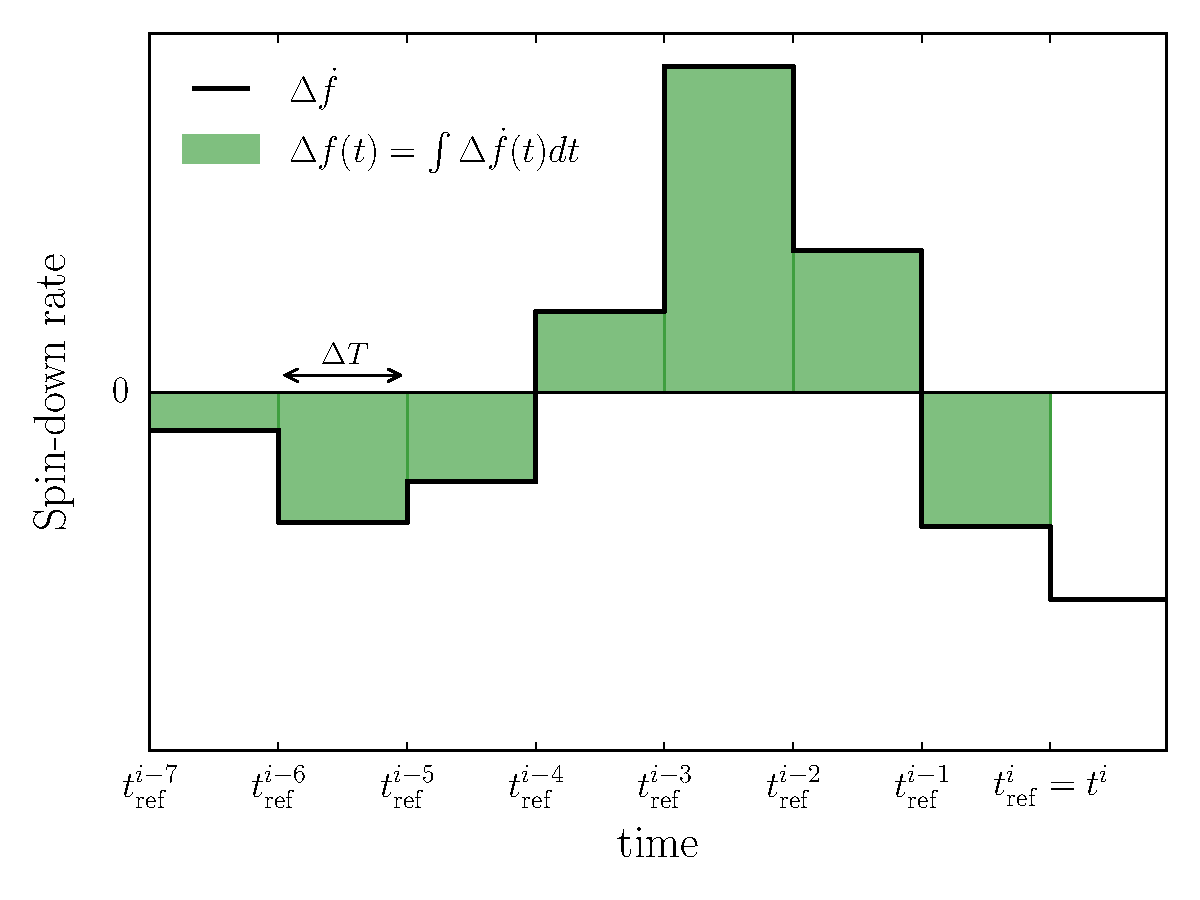
\includegraphics[width=0.7\textwidth]{Illustration_F1_int}
\caption{An example of a random walk in the spin-down rate, 
Eqn.~\eqref{eqn: delta fdot n}. The filled green blocks indicate the
summation defined in Eqn.~\eqref{eqn: f offset induced} required to
calculate the induced change in frequency at $t^{i}$ due to the random walk in
spin-down rate.}
\label{fig: Illustration fdot int}
\end{figure}

If we want to model a random walk in the phase, frequency, and spin-down rate
concurrently, then we must consider the effect that a
random walk in spin-down will have on the frequency and phase. For example, if we
increase the spin-down rate for a period of time, then we would expect the frequency
to decrease at a greater rate during this period. In our discreet model, it is
not possible to dynamically change the frequency during a single subdomain.
However, we can approximate this by updating the frequency in the next
subdomain with the induced frequency offset due to the spin-down in previous
subdomains. This must be done for the induced effect from the random walk in spin-down rate on
the phase and frequency, and for the induced effect from the random walk in frequency
on the phase. There is induced effect for the spin-down rate: the effect only
propagates to lower order terms.

Because the random walk is discreet and constant in any given subdomain, we can
calculate the offset in the lower order terms from a Taylor expansion. The
total offset at the  $i^{th}$ reference time is then given by the summation of
the offset caused by all higher order terms up to that reference time. The
reference times can be arbitrarily chosen, but setting each to start at the
beginning of the subdomain simplifies the calculation. 
The frequency offset induced by the spin-down can be
calculated using a Taylor expansion
\begin{equation}
\Delta \f_{i} = \s{j=1}{i-1}\Delta\fdot_{j} \dT .
\label{eqn: f offset induced} 
\end{equation}
This can be though of as the integration of the spin-down up to the $i^{th}$
reference time and is illustrated by the green blocks in Fig.~\ref{fig:
Illustration fdot int}. 

Since we want to consider random walks in all three parameters we now add in a
random walk in frequency. Each step is independent of the induced effect from
the spin-down and is given by \mbox{$\tn \f_{i} \sim \mathcal{N}(0, \sigF)$}. The two
effects will sum linearly such that the frequency offset is
\begin{equation}
\Delta \f_{i} = \s{j=1}{i}\tn \f_{j} + \s{j=1}{i-1}\Delta\fdot_{j} \dT.
\label{eqn: f offset} 
\end{equation}

By a similar process we can calculate the induced effect of the frequency and
spin-down on the phase. Including the random walk in the phase
for which $\delta \phi_i \sim \mathcal{N}(0, \sigP)$, the phase offset is given by
\begin{equation}
\Delta\phi_{i}  =  \s{j=1}{i}\tn \phi_{j} 
+ 2\pi\left(\s{j=1}{i-1}\Delta \f_{j}\dT 
+ \frac{1}{2}\s{j=1}{i-1}\Delta \fdot_{j}\dT^{2}\right).
\label{eqn: phi offset}
\end{equation}

%Equations \eqref{eqn: f offset} and \eqref{eqn: phi offset} will allows us to
%construct the parameter space offsets in all three terms from the distibutions
%$\tn \phi_i$, $\tn \phi_i$, and $\tn \phi_i$.




\subsection{Random walk models part I}
\label{sec: Random walk models part I}
We will now calculate the mismatch for a fully-coherent search given the
random walk in phase, frequency, and spin-down rate defined in the previous
section.

Let us begin by expanding the metric-mismatch summation from Eqn.~\eqref{eqn:
mismatch}.  Writing the summations explicitly, we have
\begin{align}
\mutilde & = g_{\alpha\beta i j}\dl^{\alpha i}\dl^{\beta j}  \\
&=\s{i=1}{\Nsd}\s{j=1}{\Nsd}g_{\alpha\beta i j}\dl^{\alpha i}\dl^{\beta j}  \\
&= \s{i=1}{\Nsd}g_{\alpha\beta i i}\dl^{\alpha i}\dl^{\beta i}
+ \s{i=1}{\Nsd} \s{\substack{j=1\\ j \ne i}}{\Nsd} g_{\alpha \beta ij}\dl^{\alpha i}\dl^{\beta j}.
\end{align}
The summation has been intentionally split into terms for which the two
subdomains are the same and those for which they are different. The metric when
the reference time is at the beginning of each subdomain is given by
Eqn.~\eqref{eqn: metric equal subdomains tref 0}. By considering the metric for
the two cases, we can write the two distinct components as
\begin{equation}
g_{\alpha\beta ij} = \left\{
\begin{array}{cc}
g_{\alpha\beta}^{\mathrm{E}} & \textrm{ if } i =j \\
g_{\alpha\beta}^{\mathrm{NE}} & \textrm{ if } i  \ne j
\end{array}\right.  .
\end{equation}
Then the fully-coherent metric-mismatch can be calculated from
\begin{align}
\mutilde &= \s{i=1}{\Nsd}g_{\alpha\beta}^{\mathrm{E}}\dl^{\alpha i}\dl^{\beta i}
+ 2\s{i=1}{\Nsd} \s{j=1}{i-1} g_{\alpha \beta}^{\mathrm{NE}}\dl^{\alpha i}\dl^{\beta j} .
\label{eqn: mismatch sep}
\end{align}

\subsection{Writing the parameter offsets in terms of normal distributions}
Equations~\eqref{eqn: f offset} and \eqref{eqn: phi
offset} give the offsets as functions of the offsets in higher order
parameters. In order to calculate statistical values, we now write these in terms of
the normal distributions from which the random walks are constructed.
Substituting Eqn.~\eqref{eqn: delta fdot n} into Eqn.~\eqref{eqn: f offset} and using the summation properties defined
in Appendix~\ref{sec: summation identities}, we have
\begin{align}
\Delta \f_{i}  & = \s{j=1}{i}\tn \f_{j}
+ \s{j=1}{i-1}\s{k=1}{j}\tn \fdot_{k} \dT ,  \\
& = \s{j=1}{i}\tn \f_{j}
+ \s{j=1}{i-1}(i-j)\tn \fdot_{j} \dT .
\label{eqn: delta f n}
\end{align}
Similarly, substituting this equation into Eqn.~\eqref{eqn: phi offset} we
have
\begin{align}
\begin{split}
\Delta\phi_{i} & = \s{j=1}{i}\tn \phi_{j}
+ 2\pi \left(\s{j=1}{i-1}\Delta\f_{j}\dT
+ \frac{1}{2}\s{j=1}{i-1}\Delta\fdot_{j}\dT^{2}\right) \\
& = \s{j=1}{i}\tn \phi_{j} + 2\pi\left(\s{j=1}{i-1}\left(\s{k=1}{j}\tn\f_{k}
+ \s{k=1}{j-1}(j-k)\tn\fdot_{k}\dT\right)\dT
 + \frac{1}{2}\s{j=1}{i-1}\s{k=1}{j}\Delta\fdot_{k}\dT^{2} \right)  \\
& = \s{j=1}{i}\tn \phi_{j} + 2\pi\left(\s{j=1}{i-1}(i-j)\tn\f_{j}\dT
 + \s{j=1}{i-1}\s{k=1}{j-1}(j-k)\tn\fdot_{k}\dT^{2}
 + \frac{1}{2}\s{j=1}{i-1}(i-j)\Delta\fdot_{j}\dT^{2} \right)  \\
& = \s{j=1}{i}\tn \phi_{j} + 2\pi\left(\s{j=1}{i-1}(i-j)\tn\f_{j}\dT
 + \frac{1}{2}\s{j=1}{i-1}\left(\left(i-j\right)\left(i-j-1)\right)
 + (i-j)\right)\tn\fdot_{j}\dT^{2}\right)  \\
& = \s{j=1}{i}\tn \phi_{j} + 2\pi\left(\s{j=1}{i-1}(i-j)\tn\f_{j}\dT
 + \frac{1}{2}\s{j=1}{i-1}(i-j)^{2}\tn\fdot_{j}\dT^{2}\right)
\end{split}
\label{eqn: delta phi n}
\end{align}

\subsection{Taking the expectation}

In Eqn.~\eqref{eqn: delta fdot n}, Eqn.~\eqref{eqn: delta f n},
Eqn.~\eqref{eqn: delta phi n} we have written the parameter space offsets
(which are to be used in calculating the mismatch) purely in terms of the
random walk distributions $\tn \phi_i$, $\tn \f_i$, and $\tn \fdot_i$. We can
calculate the mismatch exactly given a set of random walk jumps by inserting
these into Eqn.~\eqref{eqn: mismatch sep}. However, since we are dealing with
statistical quantities, we can instead infer the behaviour of the mismatch
under the random walk by taking an expectation.

Inserting Eqn.~\eqref{eqn: delta fdot n}, Eqn.~\eqref{eqn: delta f n},
Eqn.~\eqref{eqn: delta phi n}  in Eqn.~\eqref{eqn: mismatch sep} yields a
number of terms with all the permutations of two terms from $[\tn \phi, \tn \f,
\tn \fdot]$. Taking the expectation, all the cross-correlated terms, such as
$\tn\phi_{i}\tn \fdot$, will have an expectation of zero since the steps of the
random walk are independent. The only non-vanishing terms are given by
\begin{align}
E[\tn\phi_{i}\tn\phi_{j}] &= \delta_{ij}\sigP, &
E[\tn\f_{i}\tn\f_{j}] &= \delta_{ij}\sigF,&
E[\tn\fdot_{i}\tn\fdot_{j}] &= \delta_{ij}\sigS,
\end{align}
After some simplification we find that the mismatch is given by
\begin{align}
\begin{split}
E[\mutilde]   = &  \frac{A_{\phi}}{6} \left(\Nsd - \frac{1}{\Nsd}\right)
+ \frac{\pi^{2} A_{{f}}}{30}\left(4 \Nsd^{3} + 5 \Nsd^{2} + \frac{1}{\Nsd}\right)\\
 & +  \frac{\pi^{2} A_{{\dot{f}}}}{3780} \left(66 \Nsd^{5} - 21 \Nsd^{3} + 105 \Nsd^{2}
 + 217 \Nsd + 63 - \frac{94}{\Nsd}\right),
\end{split}
\label{eqn: expectation}
\end{align}
where
\begin{equation}
	A_{\phi} = \sigP \;\;\;\;\;
    A_{\f} = \sigF\Delta T^{2} \;\;\;\;\;
    A_{\fdot} = \sigS\Delta T^{4},
\end{equation}
define three `activity parameters'.

Recalling that $\Nsd=\Tobs/\Delta T$, Eqn.~\eqref{eqn: expectation} makes
predictions for the leading order
scaling of the three random walks with the observation period
\begin{equation}
E[\mutilde]_{\mathrm{PN}} \sim \sigP \frac{\Tobs}{\Delta T}, \hspace{10mm}
E[\mutilde]_{\mathrm{FN}} \sim \sigF \frac{\Tobs^{3}}{\Delta T}, \hspace{10mm}
E[\mutilde]_{\mathrm{SN}} \sim \sigS \frac{\Tobs^{5}}{\Delta T}.
\label{eqn: scalings}
\end{equation}

These results are a function both of the observation span $\Tobs$ and the
random walk model parameters $\sigP, \sigF, \sigS$ and $\Delta T$. In
Appendix~\ref{sec: physical interpretation of the monthly ephemeris}, we showed
that for a compound Poisson process random walk, the variance after a duration
$\Delta T$ scaled as $\sigma^{2} \propto \Delta T$. This means that the leading
order scalings in Eqn.~\eqref{eqn: scalings} are insensitive to how the random
walk is parameterised: changing $\Delta T$ produces a corresponding change in
$\sigma^{2}$ such that the leading order mismatch remains the same for a fixed
observation time.

\subsection{Verifying the results}

We can observe the leading order scaling of Eqn.~\eqref{eqn: scalings}
directly and verify the predictions made by Eqn.~\eqref{eqn: expectation} by
comparing with exact numerical results. That is, using the signal injection and
recovery tools developed in Section~\ref{sec: narrow-band method} of
Chapter.~\ref{sec: timing noise in cgw} we simulate signals undergoing a random
walk and calculate the corresponding mismatch (no minimisation step is done
here, this is discussed in the next section). In particular, we perform three
Monte Carlo studies for a random walk in the phase, frequency, and spin-down
rate and in each case compare the simulated results with the analytic
prediction. The results are shown in Figure~\ref{fig: rw I} and demonstrate good
agreement between the simulation means and the prediction of Eqn.~\eqref{eqn:
expectation}.

\begin{figure}[ht]
\centering
\subfloat[Random walk in phase]{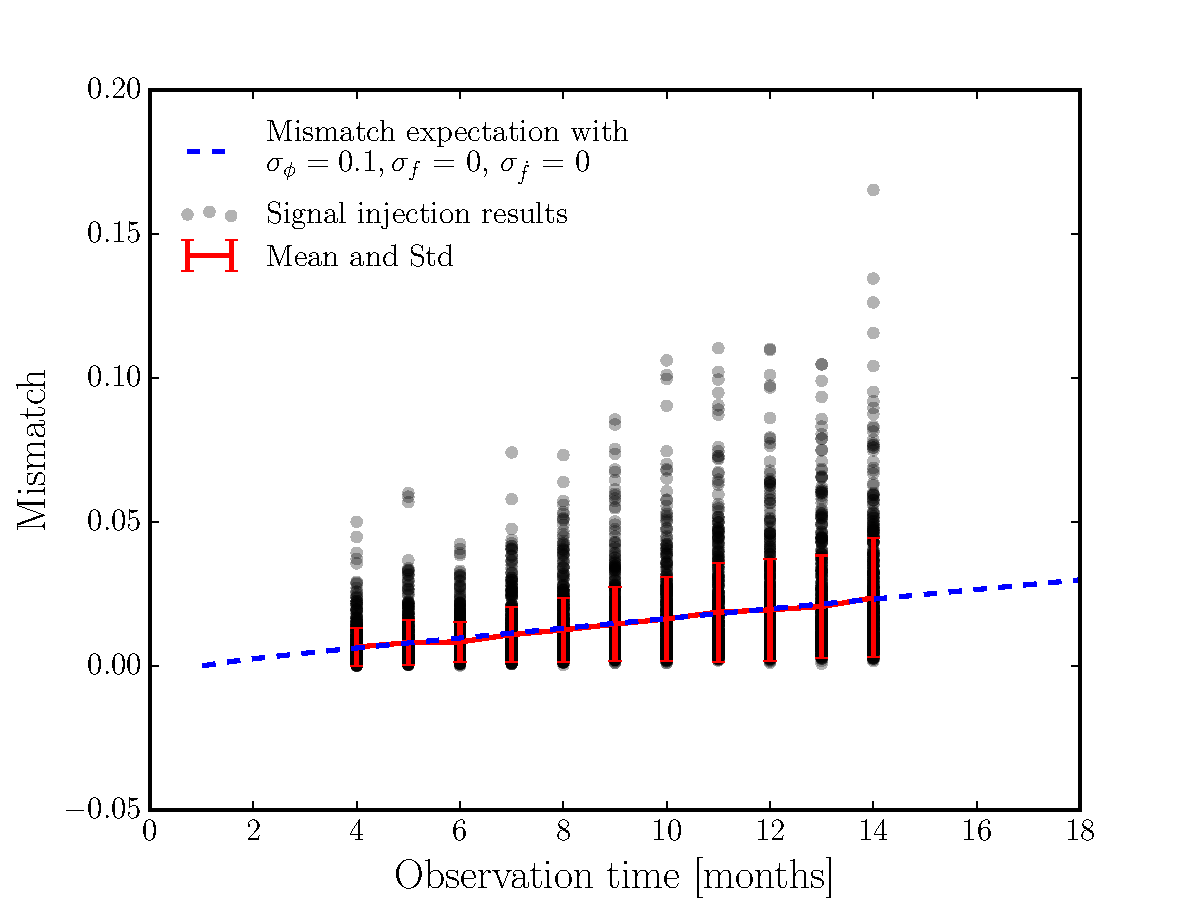
\includegraphics[width=0.5\textwidth]{ExpectationPhase}}
\subfloat[Random walk in frequency]{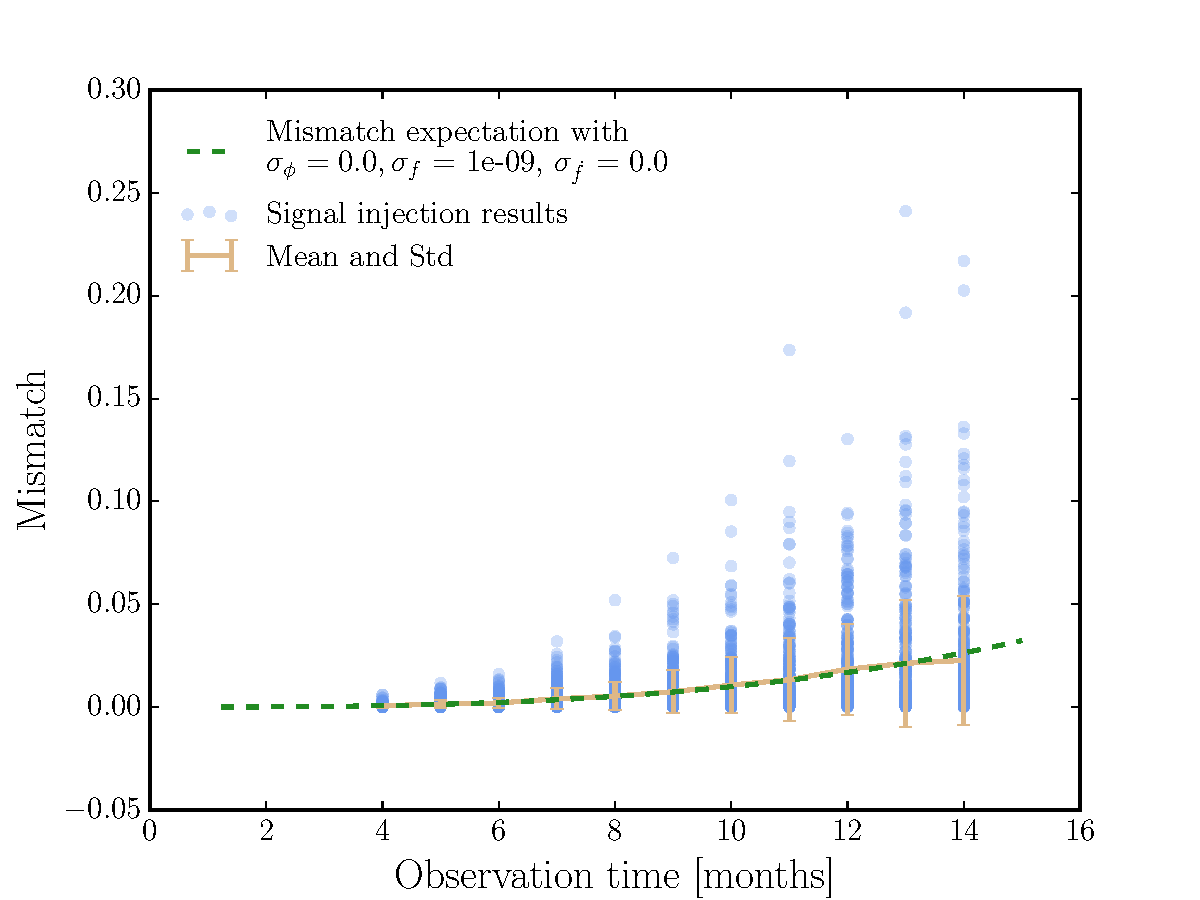
\includegraphics[width=0.5\textwidth]{ExpectationFrequency}}\\ \subfloat[Random walk in spin-down]{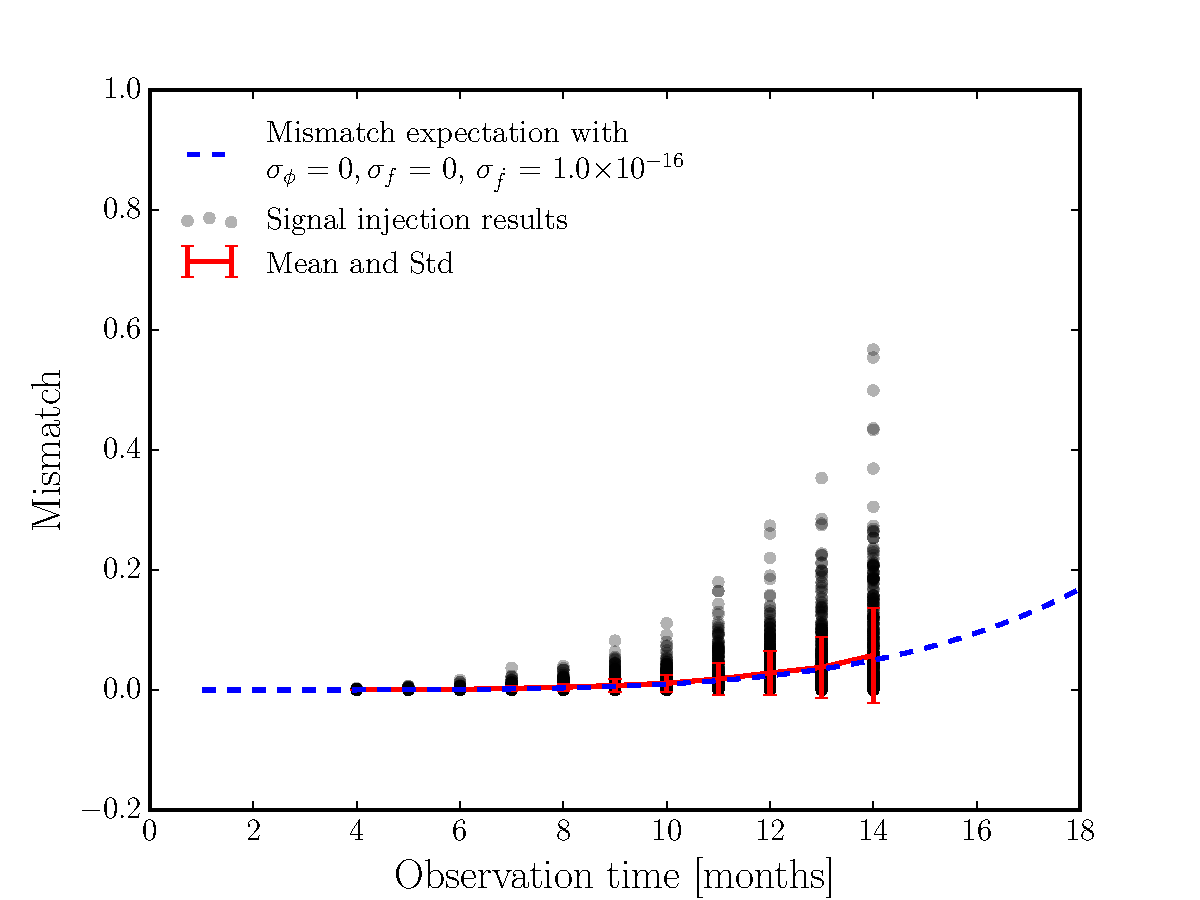
\includegraphics[width=0.5\textwidth]{ExpectationSpindown}}
\caption{A comparison of Monte Carlo numerical simulated mismatch with the prediction
of Eqn.~\eqref{eqn: expectation} for a random walk in the phase, frequency,
and spin-down rate.}
\label{fig: rw I}
\end{figure}

\subsection{Implied scalings}



\subsection{Random walk models part II} 
\label{sec: Random walk models part II}
In Section~\ref{sec: Defining a random walk} we have defined a random walk
model for which we subsequently calculated the fully-coherent mismatch in
Section~\ref{sec: Random walk models part I}. However, this is a special case
in which the random walk for each parameter offset (the difference between the
signal and the template) begins at the origin and then grows with time. It is
the signal which undergoes a random walk, so in this case we have set the
template to exactly match the signal and $t=0$. However, one could imagine choosing
the template in a different way which would reduce the overall mismatch; as such
Eqn.~\eqref{eqn: expectation} may overestimate the mismatch. The proper thing to
do is to minimise the mismatch with respect to the
template parameters~$\lt^{\alpha}$ which are implicitly in the calculation of
Section~\ref{sec: random walk models part I} through
\begin{align}
\Delta \lambda^{\alpha i} = \ls^{\alpha i} - \lt^{\alpha i},
\end{align}
as first defined in Section~\ref{sec: generalising the metric mismatch}.

Ideally, we would like to repeat the calculation leading to Eqn.~\eqref{eqn:
expectation} minimising the mismatch with respect to the template parameters.
However, this calculation has not yet been peformed so a practical alternative
method which we will use here is to begin with the random walk starting at the
origin, as defined in Section~\ref{sec: Defining a random walk}, and then fit and
remove a polynomial of degree $k$. This leaves us with a residual random walk for
which we then compute the mismatch. We will then verify that this captures the
essential features of minimising the mismatch by comparing with numerical
simulations in which the exact mismatch is minimised numerically.

In Appendix~\ref{sec: least squares minimisation of a random walk}, we
introduce the basic tools of least squares fitting and removing a polynomial of
degree $k$ to a generic random walk. In the following sections, we will
calculate the minimised mismatch for random walks in the phase or frequency; we
have not yet calculated the corresponding result for mixtures or random walks
in the spin-down rate. We have a choice in the degree of polynomial to fit and
remove. Since most searches minimise the mismatch with respect to the template
frequency $f_\textrm{t}$ and spin-down rate $\dot{f}_{\textrm{t}}$, this is
equivalent to fitting and removing a $k=2$ polynomial to the phase residual.

\subsection{Random walk in the phase}
\label{sec: minimised rw in phase}
We begin with the simplest case of a random walk in phase, for which we have
\begin{equation}
\Delta\phi_{i} = \s{j=1}{i}\mathcal{N}(0, \sigP).
\end{equation}
Then, as shown in Eqn.~\eqref{eqn: E yiyi} of Appendix~\ref{sec: least squares
minimisation of a random walk}, we have that
\begin{equation}
E[\Delta\phi_{i} \Delta\phi_{j}] = \sigP \min(i, j).
\end{equation}

Then, we define the residual difference between the signal and template
after fitting and removing a $2^{nd}$ order polynomial, $\hat{y}_i^{(2)}$, as
\begin{align}
\Delta^{(2)}\phi_i = \Delta\phi_i - \hat{y}_i^{(2)}.
\label{eqn: D2phi}
\end{align}
Note that the superscript `(2)' indicates the degree of polynomial and by
$\Delta^{(2)}\phi_i$ we mean the residual difference between the signal and
template after fitting and removing the polynomial.

We set the difference between the signal and template in all other parameters
to zero such that the mismatch for a random walk in the residual phase is
therefore
\begin{align}
\mutilde & = g_{0 0 i j} \Delta^{(2)}\phi^{i}\Delta^{(2)}\phi^{j} \\
& = \s{i=1}{\Nsd}g_{00}^{E} \Delta^{(2)}\phi_{i}\Delta^{(2)}\phi_{i}
+ 2 \s{i=1}{\Nsd}\s{j=1}{i-1}g_{00}^{NE}\Delta^{(2)}\phi_{i}\Delta^{(2)}\phi_{j}.
\label{eqn: 4202540871}
\end{align}
To calculate the expectation of the mismatch, we need to evaluate the
expectation of
\begin{align}
\Delta^{(2)}\phi_{i}\Delta^{(2)}\phi_{i} = & \left(\Delta\phi_{i}
- \s{k=1}{\Nsd}\CT_{ik}\Delta\phi_{k}\right)
 \left(\Delta\phi_{j} - \s{l=1}{\Nsd}\CT_{jl}\Delta\phi_{l}\right) \\
= & \Delta\phi_{i}\Delta\phi_{j} -
\left(\s{k=1}{\Nsd}\CT_{ik} \Delta\phi_{j}\Delta\phi_{k}
+ \s{l=1}{\Nsd}\CT_{jl}\Delta\phi_{i}\Delta\phi_{l}\right) \nonumber \\
& +
\s{k=1}{\Nsd}\s{l=1}{\Nsd}\CT_{ik}\CT_{jl} \Delta\phi_{k}\Delta\phi_{l},
\end{align}
where $\CT_{ij}$ is defined in Eqn.~\ref{eqn: C_2} and Eqn.~\ref{eqn:  MCC_2}
of Appendix~\ref{sec: least squares minimisation of a random walk} and we have
replaced $\Delta x$ with the time $\dT$. Then taking the expectation
\begin{align}
\E{\Delta^{(2)}\phi_{i}\Delta^{(2)}\phi_{i}} & =
%E\left[\Delta\phi_{i}\Delta\phi_{j}\right] -
%\left(\s{k=1}{\Nsd}E[\Delta\phi_{j}\Delta\phi_{k}]
%+ \s{l=1}{\Nsd}E[\Delta\phi_{i}\Delta\phi_{l}]\right) +
%\s{k=1}{\Nsd}\s{l=1}{\Nsd}E[\Delta\phi_{k}\Delta\phi_{l}]\\
%& = 
\sigma^{2}_{\phi} \left(\min(i, j) - \left(\s{k=1}{\Nsd}\CT_{ik} \min(j, k)
+ \s{l=1}{\Nsd}\CT_{jl}\min(i, l) \right)\right. \notag \\
& \hspace{13mm} \left. + \s{k=1}{\Nsd}\s{l=1}{\Nsd}\CT_{ik}\CT_{jl}\min(k, l)\right).
\label{eqn: expected mismatch dP0idP0j_k2}
\end{align}
Using symbolic mathematics packages we
calculate an analytic expression which is a function of $\dT, i, j$ and $\Nsd$.
Inserting this into Eqn.~\eqref{eqn: 4202540871} and simplifying we find that
\begin{align}
E[\mutilde]  & = \s{i=1}{\Nsd}g_{00}^{E} E\left[\Delta^{(2)}\phi_{i}\Delta^{(2)}\phi_{i}\right]
+ 2 \s{i=1}{\Nsd}\s{j=1}{i-1}g_{00}^{NE}E\left[\Delta^{(2)}\phi_{i}\Delta^{(2)}\phi_{j}\right]  \\
& = \frac{1}{70}\sigP\left(3N - \frac{27}{\Nsd}\right).
\label{eqn: Expected mismatch RW in phase k2}
\end{align}
This expression can be compared to Eqn.~\eqref{eqn: expectation} ignoring the
effect of the random walk in spin-down rate. Notably, we retain the same
leading order scaling of $\Nsd$, but the overall coefficient is decreased.
Rearranging the expression in the bracket demonstrates the mismatch is negative
or zero for $1 \ge \Nsd \ge 3$: this is a reflection of the minimum number of
points needed in order to perform the quadratic fit. This is shown later in
Sec.~\ref{sec: appendix conclusions} for the simpler case of fitting and
removing a polynomial from a generic random walk.

\subsection{Random walk in the frequency}

For a random walk in the frequency we have an added complexity caused by the
effect the frequency offsets induces in the phase. For the frequency offset we
have
\begin{align}
\Delta f_{i} &= \s{j=1}{i}\mathcal{N}(0, \sigF).
\end{align}
Recalling that we set the reference time at the beginning of each subdomain,
then as in Section~\ref{sec: Defining a random walk}, the induced phase offset is
\begin{align}
\Delta\phi_{i} &=2\pi \s{j=1}{i-1}\Delta f_{j}\dT \\
 & = 2\pi\dT \s{j=1}{i-1}\s{k=1}{j}\mathcal{N}(0, \sigF) \\
& = 2\pi\dT \s{j=1}{i}(i-j)\mathcal{N}(0, \sigF).
\label{eqn: P2F}
\end{align}
Note that we do not include a random walk in the phase here.

Then we calculate the expected values of combinations of the parameter space
offsets
\begin{align}
E[\Delta\f_{i}\Delta\f_{j}] & = \sigF \min(i, j), \label{eqn: E1} \\
E[\Delta\phi_{i}\Delta\f_{j}] & = 2 \pi \dT \sigF \s{k=1}{\min(i, j)}(i-k), \label{eqn: E2}\\
E[\Delta\phi_{i}\Delta\phi_{j}] & =
\left(2\pi\dT\right)^{2}\sigF \s{k=1}{\min(i, j)}(i-k)(j-k).
\label{eqn: E3}
\end{align}

In Eqn.~\eqref{eqn: D2phi}, we defined the residual difference between the signal
and template phase after fitting and removing a scond order polynomial. The
second order polynomial was chosen to model the effect of minimising over the
template frequency and frequency derivative. Let us now define
\begin{align}
\Delta^{(1)}f_i = \Delta f_i - \hat{y}^{(1)},
\label{eqn: D2f}
\end{align}
as the residual difference between the signal and template frequency after
fitting and removing a first order polynomial. In this instance, the first
order polynomial models the effect of minimising over the template
frequency and frequency derivative.

To calculate the mismatch, we expand Eqn.~\eqref{eqn: mismatch} summing over
the residual frequency offset $\Delta^{(1)}f_i$ (defined in Eqn.~\eqref{eqn:
D2f}) and the residual phase offset $\Delta^{(2)}\phi_i$ (given by
subsituting Eqn.~\eqref{eqn: P2F} into Eqn.~\eqref{eqn: D2phi}), this gives
\begin{align}
\begin{split}
E[\mutilde] = &
\s{i=1}{\Nsd}\left(g_{00}^{E}E\left[\Delta^{(2)}\phi_{i}\Delta^{(2)}\phi_{i}\right]
+ 2 g_{01}^{E}E\left[\Delta^{(2)}\phi_{i}\Delta^{(1)}\f_{i}\right]
+  g_{11}^{E} E\left[\Delta^{(2)}\f_{i}\Delta^{(1)}\f_{i}\right] \right) \\
& + 2\s{i=1}{\Nsd}\s{j=1}{i-1}\left(\right.
g_{00}^{NE}E\left[\Delta^{(2)}\phi_{i}\Delta^{(2)}\phi_{j}\right] +
g_{01}^{NE}E\left[\Delta^{(2)}\phi_{j}\Delta^{(2)}\f_{i}\right] +  \\
&\hspace{20mm}\left. g_{10}^{NE}E\left[\Delta^{(2)}\phi_{i}\Delta^{(2)}\f_{j}\right] +
g_{11}^{NE} E\left[\Delta^{(1)}\f_{i}\Delta^{(1)}\f_{j}\right] \right).
\end{split}
\end{align}


We calculate each of these expressions in a similar manner to Eqn.~\eqref{eqn:
expected mismatch dP0idP0j_k2} replacing the relevant expectations with those
given in Eqn.~\eqref{eqn: E1} to Eqn.~\eqref{eqn: E3}. This yields an expected
mismatch given by
\begin{equation}
E[\mutilde] = \frac{\pi^{2} }{630} \sigF \dT^{2}  \left(\Nsd^{3} + 13\Nsd + \frac{82}{\Nsd} \right).
\label{eqn: Expected mismatch RW in frequency k2}
\end{equation}
This can be compared with the frequency noise term alone in Eqn.~\eqref{eqn:
expectation}. We note that the leading order power remains unchanged, but there
is a reduction in the coefficient and a difference in the second highest
power. The reduction in the coefficient is expected since we have minimised
the mismatch; the change in the second highest power is not yet understood.

\subsection{Verification}

We now verify Eqn.~\eqref{eqn: Expected mismatch RW in frequency k2} and
Eqn.~\eqref{eqn: Expected mismatch RW in phase k2} by comparing with Monte
Carlo simulations. The numerical signals undergo a random walk as described in
Section~\ref{sec: Random walk models part I}, however, when searching for the
signals we search over a grid of points in $f_\textrm{t}$ and
$\dot{f}_\textrm{t}$ then select grid point with the minimum mismatch; this
minimises the mismatch over the frequency and spin-down. The results are
plotted in Figure~\ref{fig: verification of minimised RW} and demonstrate good
agreement between the analytic prediction and the mean of the simulated
mismatches.

\begin{figure}[ht]
\centering
\subfloat[Random walk in phase]{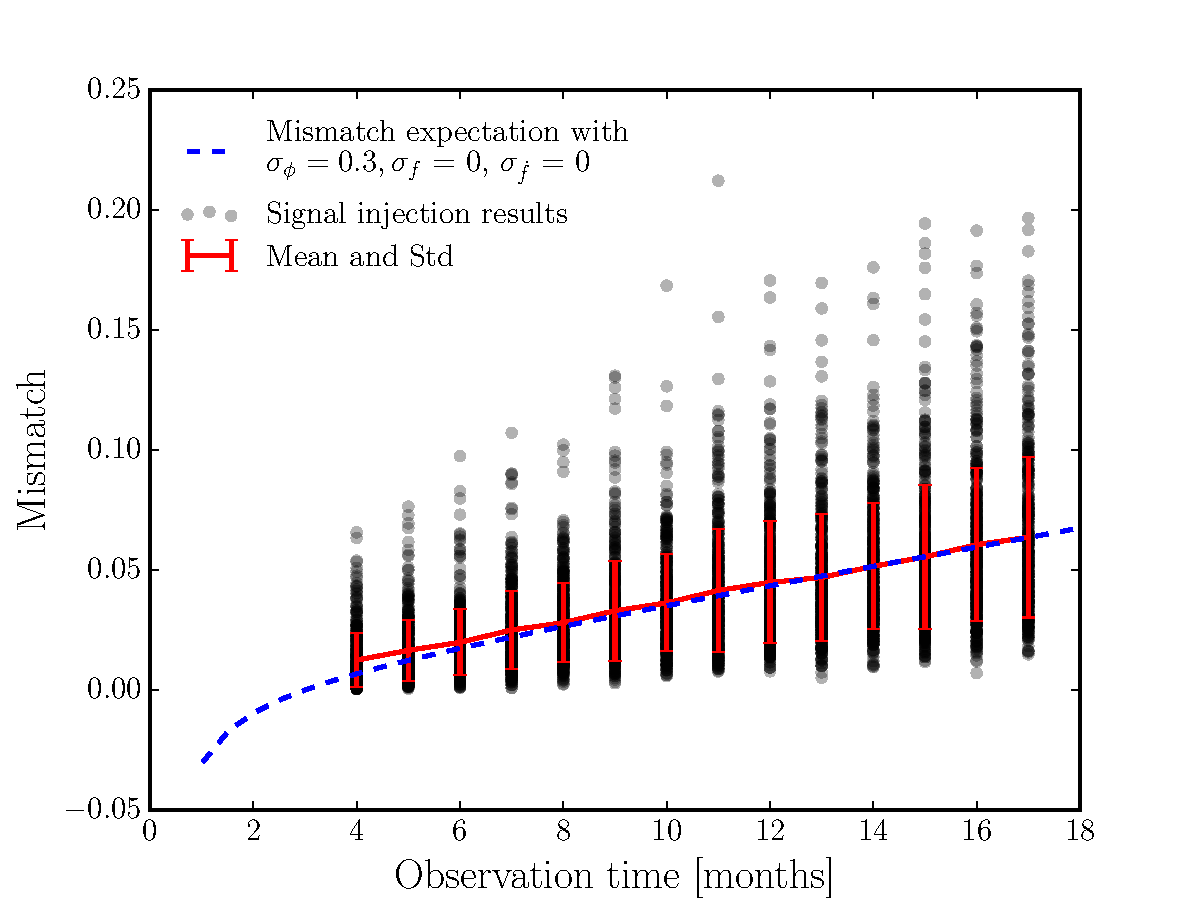
\includegraphics[width=0.5\textwidth]{ExpectationPhase_NarrowBand}}
\subfloat[Random walk in frequency]{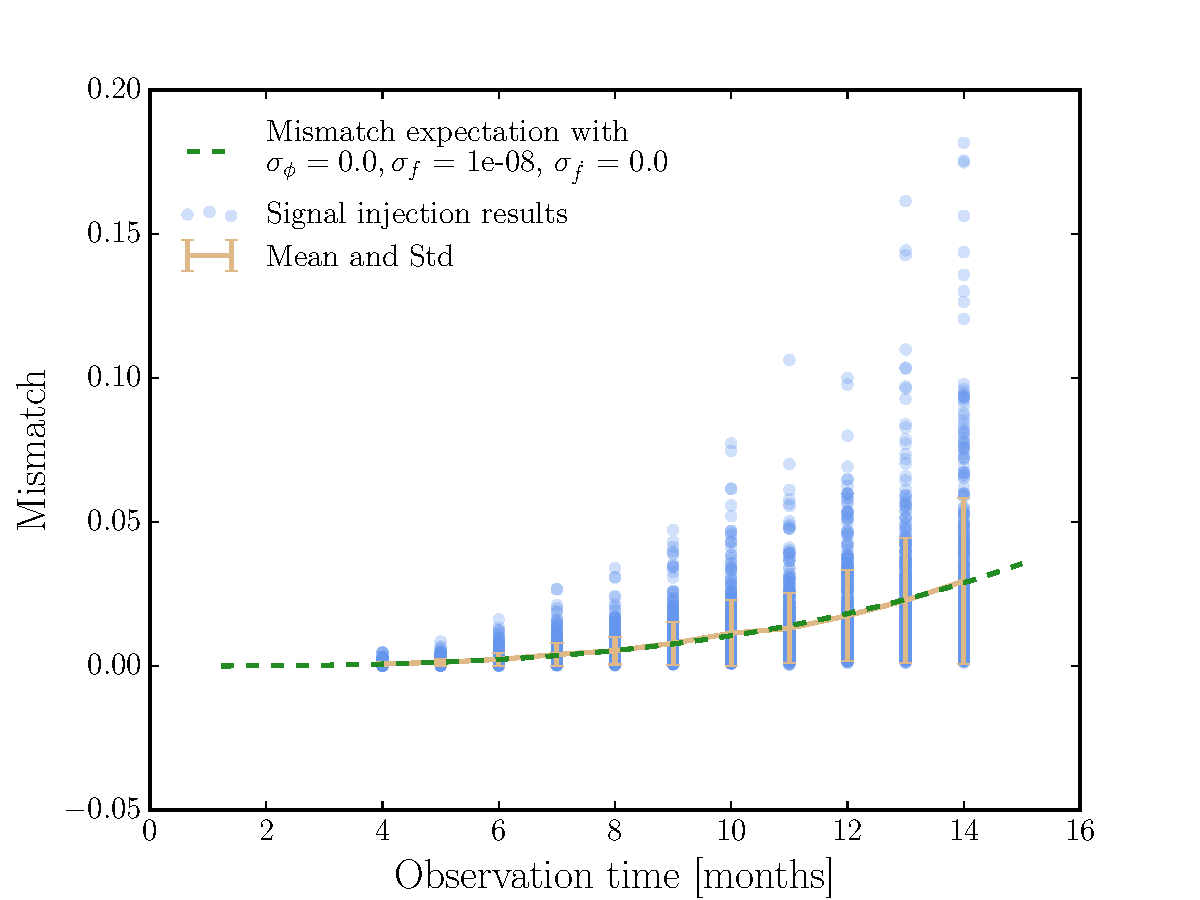
\includegraphics[width=0.5\textwidth]{ExpectationFrequency_NarrowBand}}\\
%\subfloat[Random walk in spin-down]{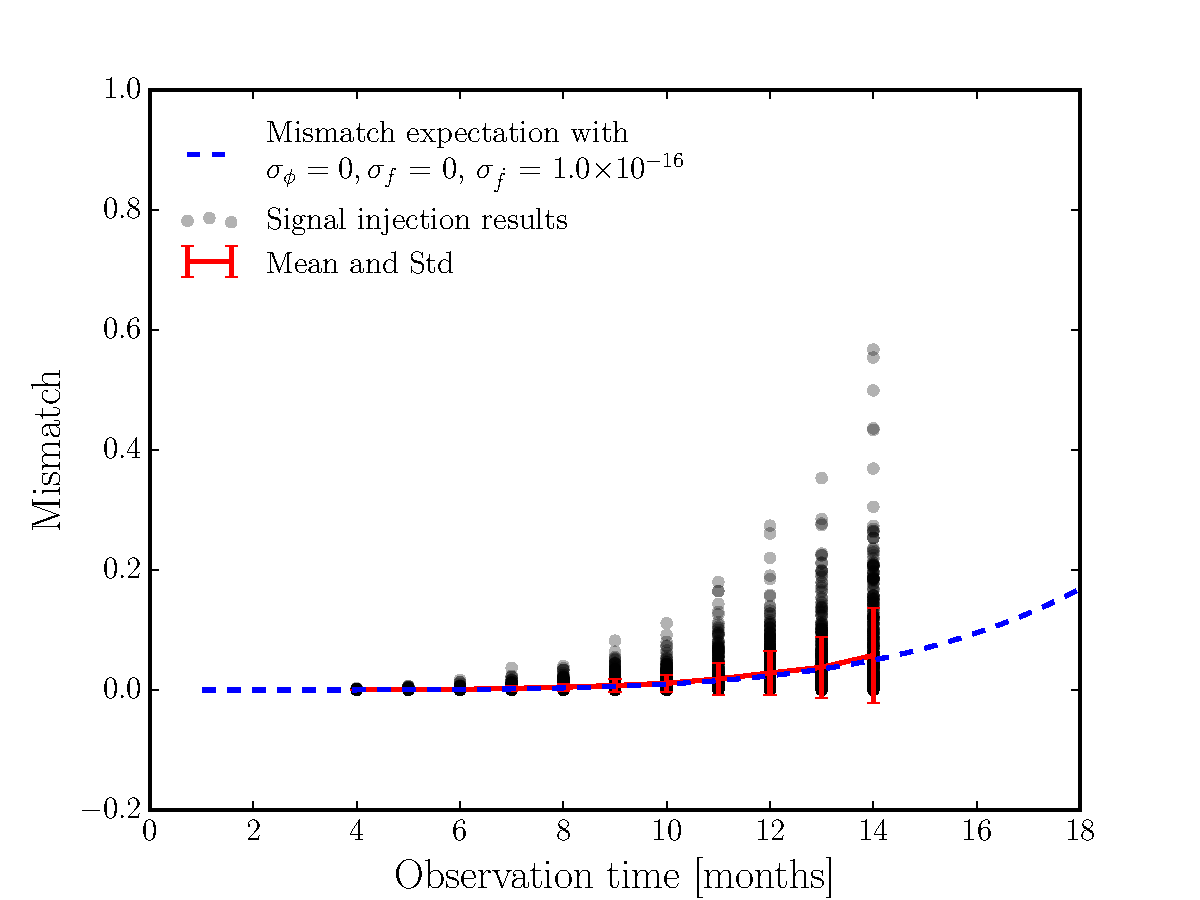
\includegraphics[width=0.5\textwidth]{ExpectationSpindown}}
\caption{A comparison of the Monte Carlo numerical simulated mismatch with the
predictions of Eqn.~\eqref{eqn: Expected mismatch RW in
frequency k2} and Eqn.~\eqref{eqn: Expected mismatch RW in phase k2}; this differs
from Figure~\ref{fig: rw I} in that the numerical mismatch is minimised by selecting
the smallest mismatch from a grid of points in $f_\textrm{t}$ and $\dot{f}_\textrm{t}$.}
\label{fig: verification of minimised RW}
\end{figure}•
\FloatBarrier


\section{Two state switching model}
\label{sec: Two state switching model}
\newcommand{\dST}{\Delta\fdot_{T}}
\renewcommand{\tref}{t_{\textrm{R}}}

\newcommand{\two}[2]{
\left\{
\begin{array}{cc}
#1  &t \in A \\
#2& t \in B
\end{array}•
\right.}

%\subsection{Calculating the mismatch}
%\textcolor{red}{Here is a derivation - better to use the mismatch framework worked out in the last chapter.}
%Having obtained the phase residual we know proceed to calculate the mismatch which would be
%induced for a CW search. 
%Initially lets consider the mismatch over a single cycle such that the observation time is $T_{\textrm{obs}} =T$.
%Then the matched filtering amplitude can be calculated by subdomaining the intergral into contribution
%when in the $A$ domain and those in $B$
%\begin{align}
%X & = \frac{1}{T}\left(\int_{A}e^{i\Delta\Phi(t)} dt + \int_{B}e^{i\Delta\Phi(t)} dt\right)
%\label{eqn: matched filtering amplitude}
%\end{align}•
%The form of the phase residual in equation~\eqref{eqn: full phase residual} does not allow for an easy integration.
%We can proceed by considering the limit  $\Delta\f_{T} \rightarrow 0$ and Taylor expand equation~\eqref{eqn: full phase residual} about this point
%\begin{align}
%\int_{A}e^{i\Delta\Phi(t)} dt & \approx \int_{0}^{RT} 1 + i\pi(1-R)t\left(t-RT\right)\dST +
%\frac{i^{2}\pi^{2}}{2}\left(1-R\right)^{2}t^{2}(t-RT)^{2}\dST^{2} dt \ntag\\
%&\approx RT - i\frac{\pi}{6} \dST R^{3}T^{3}(1-R) - \frac{\pi^{2}}{60}\dST^{2}(1-R)^{2}R^{5}T^{5}\\
%\int_{B}e^{i\Delta\Phi(t)} dt & \approx \int_{RT}^{T} 1 - i\pi R\left((t-T)(t-RT)\right) \dST+ \frac{i^{2}\pi^{2}}{2}R^{2}(t-T)^{2}(t-RT)^{2}\dST^{2} dt\\
%&\approx T(1-R) +  i\frac{\pi}{6} \dST T^{3}R(1-R)^{3} - \frac{\pi^{2}}{60}\dST^{2}T^{5}R^{2}(1-R)^{5}.
%\end{align}
%The matched filtering amplitude 
%over one cycle is then
%\begin{align}
%X &\approx 1 + i\frac{\pi}{6} \dST T^{2}\left(R(1-R)^{3} - R^{3}(1-R)\right) - \frac{\pi^{2}}{60}\dST^{2}T^{4}\left((1-R)^{2}R^{5} + R^{2}(1-R)^{5}\right) + \mathcal{O}\left(\Delta{\dot\f_{A}}^{2}\right). \\
%& \approx 1 + i\frac{\pi}{6} \dST T^{2}R\left(1-2R\right)\left(1-R\right) - \frac{\pi^{2}}{60}\dST^{2}T^{4}R^{2}(R-1)^{2}(3R^{2}-3R+1)+ \mathcal{O}\left(\Delta{\dot\f_{A}}^{2}\right).
%\end{align}
%The mismatch is then given by
%\begin{align}
%m & =1 - |X|^{2} \\
% & \approx  1 - \left|
%\left(1 - \frac{\pi^{2}}{60}\dST^{2}T^{4}R^{2}(1-R)^{2}(3R^{2} - 3R +1) \right)^{2} + \left(\frac{\pi}{6} \dST T^{2} R\left(1-2R\right)\left(1-R\right) \right)^{2}\right| \\
%& \approx \pi^{2}\dST^{2}T^{4}(1-R)^{2}R^{2}\left| \frac{1}{36}\left(1-2R\right)^{2} - \frac{1}{30}\left(3R^{2}-3R+1\right)\right| \\
%& \approx \frac{\pi^{2}}{180}\dST^{2}T^{4}(1-R)^{2}R^{2}\left|2R^{2} - 2R -1\right| 
%+ \mathcal{O}(\dST^{3})
%\label{eqn: Lyne mismatch}
%\end{align}

\subsection{Calculating the mismatch}
Writing the parameter space offsets in terms of the total spin-down variation
\begin{align}
\Delta\fdot(t) &= \dST\two{1-R}{-R} \\
\Delta\f(t) &= 0  \\
\Delta\phi(t) & = \frac{\pi}{4} \dST T^{2}(1-R)R \two{-R}{1-R},
\label{eqn: Lyne parameter space offsets}
\end{align}
note that the parameter space offsets vary discreetly with time. Combining
these into the quantity 
\begin{equation}
\bdl^{\alpha i} = \left[\bdl_{A}, \bdl_{B}\right].
\end{equation}
Then the mismatch over a single cycle can be calculated from
\begin{align}
m = & g_{\alpha\beta ij}\bdl^{\alpha i} \bdl^{\beta j},
\end{align}
where $g_{\alpha\beta i j}$ can be calculated from equation~\eqref{eqn: metric}
using the reference times for each subdomain and setting the observation time
from $t=0$ to $t=T$ (e.g. one cycle). Substituting the correct expression in we find a mismatch given by
\begin{equation}
m = \frac{\pi^{2} R^{2}}{180} T^{4} \dST^{2} \left(R - 1\right)^{2} 
    \left(-2 R^{2} + 2 R + 1\right)
\label{eqn: mismatch lyne single switch}
\end{equation}•

This is illustrated in Figure~\ref{fig: Lyne mismatch} for the valid range of R
demonstrating that the mismatch is maximal when the two periods are equal and
vanishes when either duration tends to zero as expected.

\begin{figure}[ht]
\centering
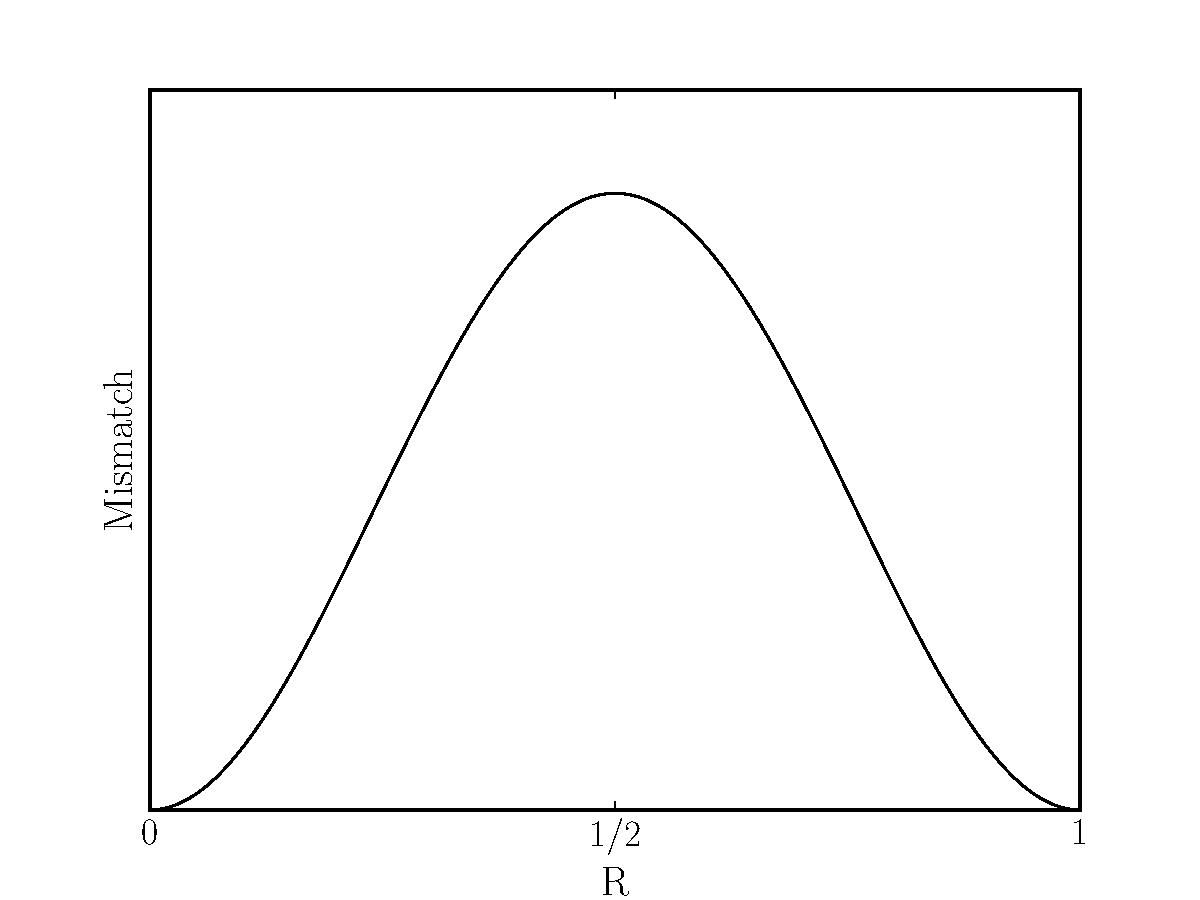
\includegraphics[width=.5\textwidth]{mismatch}
\caption{Illustration of the variation in mismatch over a single cycle with R}
\label{fig: Lyne mismatch}
\end{figure}

So far we have considered a simplistic, and highly unrealistic model. That is
measuring the mismatch over exactly one cycle. This is highly improbable in nature,
far more likely is to measure a fraction of a cycle. In Figure~\ref{fig: Lyne mismatch kappa}
such a system is illustrated having defined $\kappa$ as the fraction of a cycle that
is observed. The calculation is not reproduced as it simply requires setting 
$T_{\mathrm{obs}} = \kappa T$ when calculating the mismatch.

\begin{figure}[ht]
\centering
\includegraphics[width=.5\textwidth]{mismatch_during_one_subdomain}
\caption{Illustration of the variation in mismatch with observation time 
parameterised by $\kappa$ the fraction of a cycle that we observe over.}
\label{fig: Lyne mismatch kappa}
\end{figure}
\FloatBarrier

\subsection{Extending the model to an arbitrary number of cycles} The phase
Having calculated the mismatch during a single cycle we now extend the calculation
to an arbitary number of cycles as described by Eqn.~\eqref{eqn: arbitrary full phase residual}

The parameter
space offsets will cycle $\bdl^{\alpha i} = \left[\bdl^{A i}, \bdl^{B i}, \bdl^{A i}, \dots \bdl^{Bi}\right]$.
The metric can be decomposed into four matrices $g_{AAij}$, $g_{ABij}$, $g_{BAij}$, and $g_{BBij}$, this
allows us to expand the mismatch calculation as follows
\begin{align}
m & = g_{\alpha \beta i j} \bdl^{\alpha i} \bdl^{\beta j} \\
& = \s{i=1}{2N}\s{j=1}{2N} g_{\alpha \beta i j} \bdl^{\alpha i} \bdl^{\beta j} \\
& = N\left(\s{j=1}{2N} g_{\alpha \beta A j} \bdl^{\alpha A} \bdl^{\beta j} + \s{j=1}{2N} g_{\alpha \beta B j} \bdl^{\alpha B} \bdl^{\beta j} \right) \\
& = N^{2}\left(g_{\alpha\beta AA} \bdl^{\alpha A} \bdl^{\beta A} + g_{\alpha \beta AB} \bdl^{\alpha A} \bdl^{\beta B} + g_{\alpha \beta BB} \bdl^{\alpha B} \bdl^{\beta B} + g_{\alpha\beta BA} \bdl^{\alpha B} \bdl^{\beta A}  \right)
\end{align}
Calculating the metric elements from equation~\eqref{eqn: metric} and inserting the parameter space offsets
\eqref{eqn: Lyne parameter space offsets} yields a mismatch given by
\begin{equation}
m(T, R, N) = \frac{\pi^{2}}{180}T^{4}\dST^{2} R^{2}\left(1-R\right)^{2} \left(N \left(18 R^{2} - 18 R + 6\right) - 5 \left(2 R - 1\right)^{2}\right)
\end{equation}
This expression is valid only for searches over an integer number of cycles which is nonphysical.
The behaviour of $m$ in-between cycles will oscillate about the linear growth in $N$ that 
can be interpolated from this expression. For our purposes it is enough to see that the mismatch 
grows approximately linearly over several cycles. 



\begin{subappendices}
    \section{Summation identities}\label{sec: summation identities}
\begin{align}
\s{b=1}{c}\s{c=1}{b} X_{c} & = \left( X_{1}\right) 
 + \left( X_{1} + X_{2} \right) + \ldots  +\left( X_{1} + X_{2} 
 + \ldots + X_{c-1} + X_{c}\right)\\
& = c X_{1} + (c-1)X_{2} + \ldots + 2 X_{c-1} + X_{c} \\
& = \s{b=1}{c}(c+1-b)X_{b}
\end{align}•

\begin{align}
\s{j=1}{i-1}\s{k=1}{j-1}(j-k)X_{k} = & [0] + \left[ X_{1}\right] 
+ \left[2X_{1} + X_{2} \right] + \left[3X_{1} + 2X_{2} +X_{3}\right] 
+ \ldots  \\
& + \left[\left(i-2\right)X_{1} + \left(i-3\right)X_{2} 
+ \left(i-4\right)X_{3} + \ldots + 3X_{i-4} + 2X_{i-3} + X_{i-1}\right]  \\
= & \left(1 + 2 + 3 + \ldots +  (i-4) + (i-3) + (i-2)\right)X_{1}   \\ 
& + \left(1 + 2 + 3 + \ldots +(i-4) + (i-3) \right)X_{2}   \\ 
& + \left(1 + 2 + 3 + \ldots + (i-4) \right)X_{3} + \ldots   \\ 
& + (1 + 2 + 3)X_{i-4} + (1+2)X_{i-3} + X_{i-2}  \\
= & \s{k=1}{i-2}k X_{1} + \s{k=1}{i-3}k X_{2}  + \ldots + \s{k=1}{2}k X_{i-3} 
+ \s{k=1}{1}kX_{i-2}  \\
= & \s{j=1}{i-2}\left(\s{k=1}{i-1-j}k\right)X_{j} = 
\frac{1}{2}\s{j=1}{i-2}(i-j)(i-j-1)X_{j}
\end{align}

\end{subappendices}


\biblio

\end{document}
